\newcommand{\crel}{
	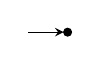
\begin{tikzpicture}[baseline={([yshift=-.8ex]current bounding box.center)}]
		\draw [->, >=stealth] (0,0) -- (0.45,0); 
		\draw [fill] (0.5,0) circle (0.05);
	\end{tikzpicture}
}

\newcommand{\rrel}{
	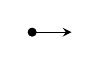
\begin{tikzpicture}[baseline={([yshift=-.8ex]current bounding box.center)}]
		\draw [fill] (0,0) circle (0.05);
		\draw [->, >=stealth] (0.05,0) -- (0.5,0);
	\end{tikzpicture}
}

\newcommand{\mrel}{
	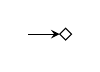
\begin{tikzpicture}[baseline={([yshift=-.8ex]current bounding box.center)}]
		\draw [->, >=stealth] (0,0) -- (0.4,0);
		\draw (0.4,0) -- (0.475,0.075) -- (0.55,0) -- (0.475,-0.075) -- cycle;
	\end{tikzpicture}
}

\newcommand{\irel}{
	\begin{tikzpicture}[baseline={([yshift=-.8ex]current bounding box.center)}]
		\draw [->, >=stealth] (0,0) -- (0.4,0);
		\draw (0.41,0) -- (0.55,0);
		\draw (0.48,-0.07) -- (0.48, 0.07); 
	\end{tikzpicture}
}

\newcommand{\erel}{
	\begin{tikzpicture}[baseline={([yshift=-.8ex]current bounding box.center)}]
		\draw [->, >=stealth] (0,0) -- (0.4,0);
		\draw (0.41,0) -- (0.55,0);
		\draw (0.48, 0.05) circle (0.02);
		\draw (0.48, -0.05) circle (0.02); 
	\end{tikzpicture}
}
